\section{Ejercicios}

\subsection{Ejercicio 1: TaskConsola}
En \'este ejercicio debemos programar una tarea \textit{TaskConsola} la cual debe realizar n llamadas bloqueantes, cada una con 
una duraci\'on al azar entre bmin y bmax, ambas pasadas por par\'ametro.

Para ello, decidimos utilizar un contador de 0 hasta n y generar un n\'umero pseudo-alaeatorio por medio de la 
funci\'on \textit{rand}. Es decir, cada vez que se aumenta el contador, realizamos una llamada bloqueante (uso\_IO) 
que durar\'a la cantidad de ciclos que se haya generado en la llamada a rand.

\subsection{Ejercicio 2: Experimentando FCFS}
Para probar el Scheduler First Came First Served usaremos el siguiente lote de tareas:

\begin{center}
TaskCPU 10\\
TaskConsola 5 1 5\\
TaskConsola 3 1 2
\end{center}

En la primera, utlizaremos TaskCPU y para darle uso intensivo correr\'a durante 10 ciclos de reloj.
Las siguientes, son de tipo TaskConsola implementado anteriormente, pas\'andole como par\'ametro el n\'umero de llamadas 
bloqueantes y el rango en el cual debe seleccionar el n\'umero aleatorio.

En el algoritmo FCFS, la CPU se asigna a los procesos en el orden en que la solicitan.\\
Por lo tanto, esperamos observar que, con un solo n\'ucleo, un proceso no pueda correr 
hasta que no terminaron los anteriores a el.

Con dos nucleos, correr\'an dos procesos simlt\'aneamente y el \'ultimo empezar\'a cuando alguno de los otros dos finalicen,
y por \'ultimo, si el procesador tiene 3 n\'ucleos, los 3 correr\'an al mismo tiempo.

\vspace{\baselineskip}
\begin{center}
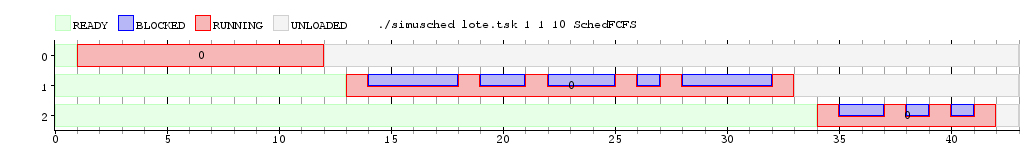
\includegraphics[scale=0.45]{../tp1/Test/resEj2Co1.png}
\\
\vspace{1pt}
\footnotesize\textit{Simulacro FCFS con un n\'ucleo}
\end{center}
\vspace{\baselineskip}


\vspace{\baselineskip}
\begin{center}
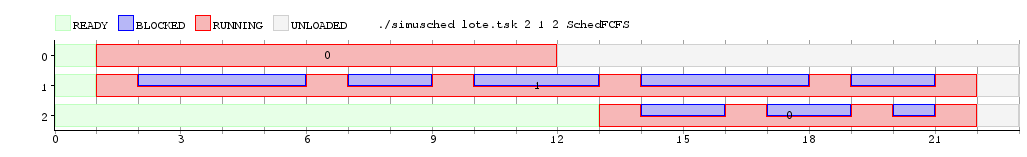
\includegraphics[scale=0.45]{../tp1/Test/resEj2Co2.png}
\\
\vspace{1pt}
\footnotesize\textit{Simulacro FCFS con dos n\'ucleos}
\end{center}
\vspace{\baselineskip}

\vspace{\baselineskip}
\begin{center}
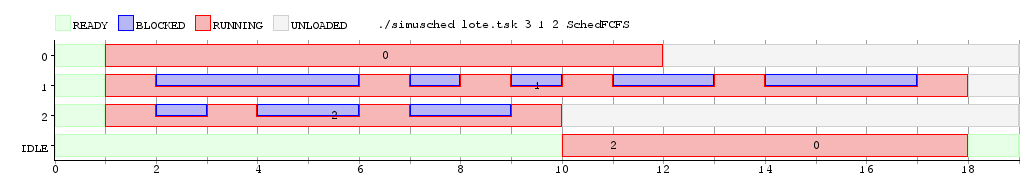
\includegraphics[scale=0.45]{../tp1/Test/resEj2Co3.png}
\\
\vspace{1pt}
\footnotesize\textit{Simulacro FCFS con tres n\'ucleos}
\end{center}
\vspace{\baselineskip}


Los experimentos corroboraron nuestra hip\'otesis, pues el comportamiento reflejado es exactamente el descripto previamente.

Adem\'as, notemos que en los casos en los que utilizamos la tarea TaskConsola, se observan claramente
las llamadas bloqueantes de manera random, dado que el tiempo tanto de la ejecuci\'on como el de las llamadas bloqueantes var\'ia.
En el caso en que el procesador tiene tres n\'ucleos, se observa que los n\'ucleos 2 y 0 ejecutan 
Idle ya que est\'an desocupadas, esperando la solicitud del pr\'oximo proceso.

\subsection{Ejercicio 3: Implementando Round-Robin}
La idea del scheduler \textit{Round-Robin} es darle un quantum a cada proceso, iterando los mismos para que todos ejecuten una vez antes de volver a comenzar la iteraci\'on.


Con esta idea desarrollamos nuestro Scheduler Round-Robin. Utilizamos como estructura una Cola $(q)$, para las llamadas a los procesos, 
un vector $(quantum)$ de tama\~no cantidad de cores del procesador que asignar\'a el quantum del i\'esimo n\'ucleo, 
y otro vector $(contador)$ que va a llevar cuenta del tiempo corrido por el proceso en el i\'esimo n\'ucleo hasta llegar al quantum del mismo.

Para el correcto funcionamiento en la funci\'on $tick$ se ven reflejados los casos en el cual el proceso debe 
dejar de correr ya sea porque termin\'o su tiempo o el quantum del procesador en el que corr\'ia. En \'este \'ultimo 
caso, la posici\'on correspondiente al n\'ucleo en $contador$ volver\'a a cero y el proceso se encolar\'a para terminar con su tiempo. 
\\Una vez realizada dicha acci\'on, debe dar lugar a la siguiente en la cola. En caso de no haber una, se ejecutara la tarea IDLE hasta el llamado de una nueva tarea.

\subsection{Ejercicio 4: Experimentando Round-Robin}

En este ejercicio nos proponemos experimentar con el scheduler del punto anterior para verificar que el comportamiento es el esperado. Haremos esto de 
manera incremental, es decir, empezaremos probando las cosas mas basicas e iremos subiendo la complejidad. 

Para empezar, probaremos RR con un solo nucleo. Notese que si le asignamos una sola tarea, su comportamiento no diferiria de alg\'un otro scheduler, por
lo que empezamos probando con cuatro tareas simultaneas. Estas tareas solo usan al cpu, por lo tanto no se bloquean. Esperamos 
verificar que el scheduler RR le asigna el tiempo del quantum a cada tarea antes de comenzar de nuevo a iterar la lista de tareas pendientes.

\vspace{\baselineskip}
\begin{center}
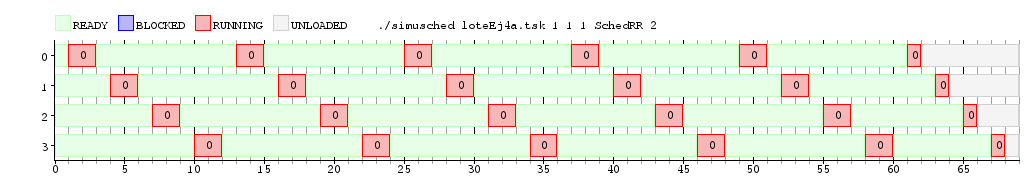
\includegraphics[scale=0.45]{../tp1/Test/resEj4Co1SB.png}
\\
\vspace{1pt}
\footnotesize\textit{Simulacro RR con un n\'ucleo}
\end{center}
\vspace{\baselineskip}

Efectivamente, cuando recibe k tareas simultaneas, el scheduler le asigna tiempo de ejecuci\'on a las tareas de modo que todas 
ejecuten antes de regresar a ejecutar la primera. 

A continuaci\'on usaremos el mismo lote de tareas, pero agregaremos otro procesador. Asi veremos si el scheduler maneja correctamente 
los procesadores para asegurarse que todas las tareas ejecuten un tiempo $quantum$ antes de volver a empezar.

\vspace{\baselineskip}
\begin{center}
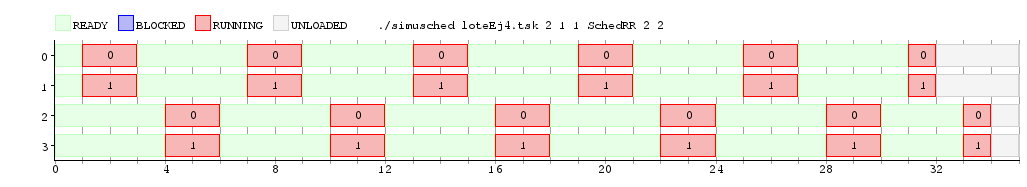
\includegraphics[scale=0.45]{../tp1/Test/resEj4Co2SB.png}
\\
\vspace{1pt}
\footnotesize\textit{Simulacro RR con dos n\'ucleo}
\end{center}
\vspace{\baselineskip}

El comportamiento es identico al anterior, solo que agregando otro nucleo, es decir, podemos deducir las mismas concluciones. Para probar de 
modo mas realista este scheduler, vamos a simular un lote de cuatro tareas que realicen llamadas bloqueantes, con dos procesadores para su ejecuci\'on.
Lo que queremos mostrar, es que el scheduler trabajara de manera optima en este caso.

\vspace{\baselineskip}
\begin{center}
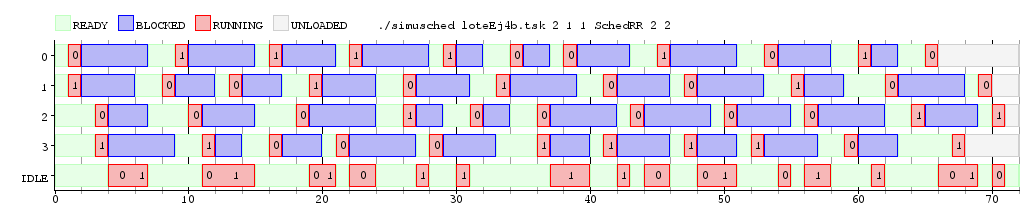
\includegraphics[scale=0.45]{../tp1/Test/resEj4Co2CB.png}
\\
\vspace{1pt}
\footnotesize\textit{Simulacro RR con dos n\'ucleo}
\end{center}
\vspace{\baselineskip}

Podemos ver que el scheduler trabaja de la manera esperada. Es decir, si hay un tarea disponible para ejecutar y procesador que no esta ejecutando nada,
ese procesador carga la tarea y la ejecuta, o bien hasta que se le acabe el quantum o hasta que se bloquee. Si todas las tareas estan bloqueadas 
o ejecutando cuando el procesador termina la ejecucion de una tarea porque se bloqueo, este se poner a ejecutar la tarea IDLE hasta que 
una tarea se desbloque. Y por lo tanto, si todas las tareas estan bloqueadas, ambos procesadores ejecutan la tarea IDLE hasta que alguna 
tarea se desbloquee.



\subsection{Ejercicio 5: \textit{Scheduling algorithms for multiprogramming in a hard-real-time environment}}
Este ejercicio est\'a dividido en dos incisos: en el primero, contestaremos una serie de preguntas formuladas por la c\'atedra, basando nuestras respuestas en el 
art\'iculo \textit{Scheduling algorithms for multiprogramming in a hard-real-time environment}; en el segundo, explicaremos el dise\~no e implementaci\'on 
de los algoritmos de scheduling de prioridades fijas y din\'amicas presentados en dicho art\'iculo.
\subsection*{Inciso 1}
En este inciso, debemos contestar tres preguntas te\'oricas acerca de los algoritmos de scheduling propuestos en el art\'iculo previamente mencionado. Antes de 
contestar las preguntas, comenzaremos con una breve descripci\'on de las condiciones de entorno sobre las cuales los algoritmos fueron ideados.
\newline
\newline
Se cuenta con un sistema, con un conjunto de tareas destinadas a resolver, cada una, una determinada funcionalidad vital para el correcto funcionamiento
de dicho sistema. Cada una de estas tareas estar\'a asociada a un evento externo, que solicitar\'a su ejecuci\'on. Es importante destacar que las tareas no
pueden ser ejecutadas antes de que dicho evento las solicite. Adem\'as, se sabe que cada tarea tiene, por un lado, una \textit{deadline} (esto es, una cantidad
de tiempo m\'aximo en el cual su ejecuci\'on debe terminar), que se mantendr\'a constante durante toda la ejecuci\'on del sistema. Por otro lado, se sabe
que el evento que solicitar\'a la ejecuci\'on de cada tarea, solicitar\'a peri\'odicamente (esto es, el intervalo de tiempo entre dos solicitudes ser\'a
siempre el mismo y no depender\'a de la terminaci\'on de otras tareas solicitadas) la ejecuci\'on de dicha tarea y, adicionalmente, se sabe que el tiempo de 
ejecuci\'on de cada tarea (entendiendo tiempo de ejecuci\'on como la cantidad de clocks que le llevar\'ia a una tarea comenzar y terminar su ejecuci\'on si el 
procesador s\'olo tuviera que ejecutar a esa tarea) ser\'a constante. Una condici\'on extra establece la existencia de tareas no peri\'odicas: estas tareas
desplazaran del procesador a las peri\'odicas y, a diferencia de las peri\'odicas, no tendr\'an una deadline estricta para terminar. Una vez establecidas
las condiciones del sistema, estamos listos para contestar las preguntas:
\newline
\newline
\textit{a}) \textquestiondown Qu\'e problema est\'an intentando resolver los autores?
\newline
\newline
Dado un sistema que se ajuste a las condiciones de entorno previamente explicadas, los autores quieren hallar una forma heuristica de organizar la ejecuci\'on de las
tareas, a medida que estas son solicitadas, de manera tal de que todas terminen su ejecuci\'on antes de su respectiva \textit{deadline}. Para esto, los 
algoritmos presentados estar\'an basados en prioridades, es decir, c\'omo se le asignar\'a la prioridad a cada tarea variar\'a seg\'un el algoritmo. Luego, los algoritmos
de scheduling deber\'an desalojar a la tarea que est\'e ocupando el procesador si llega una solicitud para la ejecuci\'on de una
tarea m\'as prioritaria. Por lo tanto, la clave para este tipo de algoritmos estar\'a en c\'omo se le asignar\'an las prioridades a las tareas.
\newline
\newline
\textit{b}) ?` Por qu\'e introducen el algoritmo de la secci\'on 7? ?`Qu\'e problema buscan resolver con esto?
\newline
\newline
Los autores introducen el algoritmo de la secci\'on 7, buscando bajar la cota superior de ln 2 sobre el tiempo de utilizaci\'on del procesador establecida 
por el algoritmo de scheduling con prioridades fijas, sin tener que asumir ninguna hip\'otesis extra para los tiempos de ejecuci\'on de las tareas, ni tampoco 
necesitar relajar las \textit{deadlines} de las tareas menos prioritarias seg\'un el esquema anterior. Para lograr esto, introducen el algoritmo de 
scheduling con prioridades asignadas din\'amicamente; es decir, a lo largo de la ejecuci\'on del sistema, las prioridades de las tareas no estar\'an
necesariamente fijas.
\newline
\newline
\textit{c}) Explicar coloquialmente el significado del teorema 7.
\newline
\newline
El teorema 7 establece una condici\'on necesaria y suficiente, sobre el algoritmo de prioridades din\'amicas, para que todas las tareas terminen de ejecutarse
antes de su \textit{deadline}. Dicha condici\'on es la siguiente:

\begin{equation*}
 C_{1}/T_{1} + ... + C_{n}/T_{n} \leq 1
\end{equation*}

donde
\begin{itemize}
  \item $n:=$ n\'umero de tareas en el sistema
  \item $C_{i}:=$ tiempo de ejecuci\'on de la tarea i\'esima
  \item $T_{i}:=$ tiempo entre dos solicitudes consecutivas por la tarea i\'esima (tambi\'en llamado per\'iodo)
\end{itemize}

Es importante se\~nalar que la condici\'on que establece este teorema nos permitir\'a, dado un lote de tareas dise\~nado para nuestros experimentos, definir 
si el algoritmo de scheduling con propiedades din\'amicas lograr\'a que todas las tareas terminen de ejecutar antes de sus respectivas \textit{deadlines}, a lo 
largo de toda la simulaci\'on.

\subsection*{Inciso 2}

En este inciso explicaremos brevemente en qu\'e consiste cada algoritmo de scheduling, y luego el dise\~no y la implementaci\'on de cada uno.

Como su nombre indica, el algoritmo de scheduling con prioridades fijas le asignar\'a a las tareas una prioridad que se mantendr\'a fija a lo largo de 
toda la ejecuci\'on del sistema. Concretamente, una tarea ser\'a m\'as prioritaria que otra cuando su per\'iodo, lease el tiempo constante transcurrido entre
dos solicitudes por dicha tarea, sea el menor de los dos. O equivalente, que su \textit{request rate}, definido como el inverso multiplicativo del per\'iodo,
sea mayor. 

Para el dise\~no de este algoritmo de scheduling, optamos por utilizar una cola de prioridad, que contendra duplas de la forma 
$<periodo(pid),pid>$, donde el m\'as prioritario ser\'a el que tenga menor per\'iodo. Este dise\~no nos permitir\'a obtener de manera sencilla cu\'al es
la pr\'oxima tarea a ser ejecutada, aprovechando las funcionalidades ya implementadas en la clase \textit{priority queue} para encolar elementos y obtener
el m\'as prioritario. De esta manera, obtener en cada tick de reloj cu\'al es la tarea a ejecutarse se resumir\'a a verificar, en primer lugar, si la 
cola de prioridad est\'a vac\'ia. En caso de que est\'e vac\'ia, se ejecutar\'a la tarea IDLE; en caso contrario, se obtendr\'a el \textit{pid} de la 
pr\'{o}xima tarea a ser ejecutada mediante la funci\'on \textit{top()}, devolviendo el segundo componente de la dupla devuelta por dicha funci\'on.

A diferencia del algoritmo anterior, el algoritmo de scheduling con prioridades din\'amicas, le asignar\'a las prioridades a cada tarea en cada
\textit{tick} de reloj. Esto se hara de la siguiente manera: a cada momento de la ejecuci\'on del sistema, la tarea m\'as prioritaria ser\'a la que
tenga su \textit{deadline} m\'as pr\'oxima; coloquialmente, esto quiere decir que lo m\'as urgente ser\'a lo m\'as prioritario. Para el dise\~no de
este scheduler, como deb\'iamos actualizar las prioridades en todos los \textit{ticks} de reloj, optamos por utilizar arreglos en vez de una cola de 
prioridad. Esto es porque, de utilizar una cola de prioridad, ser\'ia m\'as complicado iterar los procesos contenidos en la tabla para actualizar sus prioridades.
Por lo tanto, contaremos con los siguientes arreglos:

\begin{itemize}
  \item \textit{int deadline[totaltasks]} indicara, para la tarea i\'esima, cu\'anto tiempo le queda antes de su \textit{deadline} en $deadline[i]$. Para las tareas
  no peri\'odicas, adoptamos la convenci\'on de almacenar un -1 en esa posici\'on del arreglo.
  \item \textit{bool ready[total tasks]} indicar\'a, para la tarea i\'esima, si est\'a lista para correr o no.
\end{itemize}

Adicionalmente, implementaos la funcion \textit{int tareasready()}, que devolver\'a la cantidad de tareas en estado \textit{ready}.
Para obtener, en cada \textit{tick} de reloj, la pr\'oxima tarea a ejecutarse, implementamos una funci\'on de acuerdo a la siguiente l\'ogica:
Si est\'a corriendo una tarea no peri\'odica, seguir ejecutando esa. En caso contrario, verificar, en primer lugar, si hay alguna tarea
no peri\'odica en estado \textit{ready}. En caso de haberla, pasar a ejecutar esa; en caso contrario, buscar la tarea peri\'odica en estado
\textit{ready} cuya \textit{deadline} est\'e m\'as pr\'oxima y devolver esa. Vale la pena aclarar
que adem\'as, en cada \textit{tick} de reloj, se decrementar\'a el valor contenido en el arreglo \textit{deadline} para cada tarea peri\'odica que est\'e
lista para ejecutarse. En este punto, hacemos la aclaraci\'on de que hemos dejado fuera de la descripci\'on algunos de los casos borde para los cuales no 
haya tareas listas para ejecutarse, en que deba devolverse el \textit{pid} de la tarea Idle, ya que no suma a la comprensi\'on del caso en que el algoritmo
deba buscar, entre las tareas existentes, la m\'as prioritaria.

\subsection{Ejercicio 6: TaskBatch}

En este ejercicio implementamos la tarea TaskBatch, que recibe como parametros totalcpu y cantbloqueos. Esta tarea dura totalcpu tiempo de 
cpu, y realiza cantbloqueos llamadas bloqueantes en momentos psudoaleatorios. Implementamos esta tarea de dos maneras. La primera implementaci\'on itera totalcpu
veces pidiendo un numero aleatorio rand. Si rand > 0.5 entonces llama a una tarea bloqueante, sino, a una tarea que use el cpu. Si la cantidad 
de iteraciones se acaba sin haber realizado todas las llamadas bloqueantes, entonces se realizaban las restantes seguidas al final. Sino, cuando se realizaba
la ultima llamada bloqueante, se utilizaba el tiempo restante del cpu todo junto. Lo que observamos en esta implementacion fue que las llamadas bloqueantes
se hacian para tiempos grandes siempre al principio del intervalo de uso del cpu, y para tiempos de medianos a cortos, siempre al final.

Por eso realizamos otra implementacion. En esta se seleccionan previamente en que momentos se van a realizar las llamadas bloqueantes, marcando en un arreglo de totalcpu posiciones los momentos en los que se va
a llamar la tarea bloqueante. Se decide los momentos de bloqueo eligiendo un numero aleatorio entre 0 y totalcpu, asegurandonos de que no halla repetido. 
Finalmente iteramos este arreglo y llamamos a UsoIO si debemos hacer un bloqueo y a Uso CPU sino.


\subsection{Ejercicio 7}
En el siguiente ejercicio, se nos pide escoger distintas m\'etricas para poder analizar el rendimiento de el Shcheduler Round Robin para tareas de tipo TaskBatch.\\
A continuaci\'on, daremos algunos detalles de las seleccionadas.\\

\textbf{\underline{Fariness}}\\
Medimos que cada proceso reciba una dosis "justa" de CPU. Es decir, todos los procesos deben correr la misma cantidad de tiempo, en el caso de Round Robin, podemos decir el quantum que se le asigna a los procesos sea el mismo en todos los casos.\\

\textbf{\underline{Tiempo de Respuesta}}\\
En este caso, seria el tiempo que tarda una tarea en empezar a ejecutarse.
Cuanto tiempo permanece en estado ready hasta la primera ejecucion.
En el caso de Round Robin, esto depende de cuantas tareas hay esperando antes de la misma, ya que en este Scheduler se utiliza una cola como estructura, y ademas de cuantos nucleos tiene el procesador.\\

\textbf{\underline{Throughput}}\\
Son la cantidad de procesos que terminan por unidad de tiempo.\\
Esto dependera de la cantidad de bloqueos que tenga cada proceso y como se organiza la CPU en cuanto a quantum y cantidad de nucleos.\\

\textbf{\underline{Turnaround}}\\
Es el tiempo total que le toma a un proceso su ejecucion completa, contando bloqueos y cantidad de corridas en quantums de algun nucleo del CPU.

\vspace{1 cm}
Para empezar, tomaremos una CPU con un solo nucleo y con un quantum de 3 clocks.\\

\vspace{\baselineskip}
\begin{center}
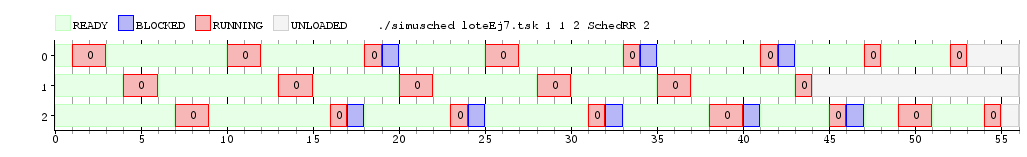
\includegraphics[scale=0.45]{../tp1/Test/resEj7Co1.png}
\\
\vspace{1pt}
\footnotesize\textit{Simulacro RR con un n\'ucleo de quantum 3}
\end{center}
\vspace{\baselineskip}

<<<<<<< HEAD
=======
Como podemos observar y ya evaluamos en ejercicios anteriores el Scheduler Round Robin funciona como lo esperado.
Ahora,nos detallaremos en su rendimiento segun las metricas detalladas anteriormente.

Si utilizamos la metrica \textit{Fairness}, este tipo de Scheduler con un solo nucleo es apropiado ya que todos los procesos recibiran la misma cantidad de tiempo de ejecucion.
Sin embargo, si nos basamos en \textit{Tiempo de respuesta} o \textit{Turnaround}, no es optimo ya que, al tener un solo nucleo, van a demorar mas tiempo en comenzar a ejecutarse y en finalizar por completo.

Ahora nos preguntamos que pasaria si aumentamos lacantidad de nucleos del procesador.
De esta manera pueden suceder dos cosas,la primera que tengan la misma cantidad de quantum ambos nucleos, y la segunda que sean distintos.
A continuacion, estudiaremos ambos casos.\\
\vspace{\baselineskip}
\begin{center}
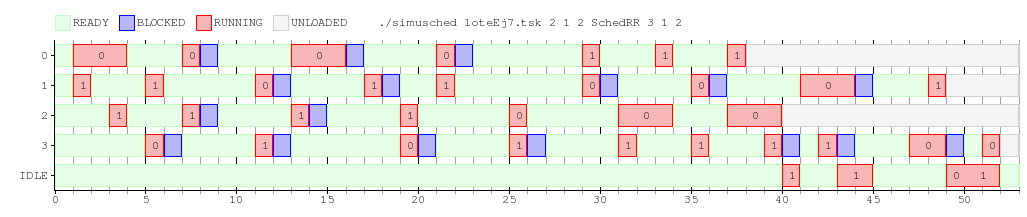
\includegraphics[scale=0.45]{../tp1/Test/resEj7Co2.png}
\\
\vspace{1pt}
\footnotesize\textit{Simulacro RR con dos n\'ucleos de quantum iguales a 3}
\end{center}
\vspace{\baselineskip}

\vspace{\baselineskip}
\begin{center}
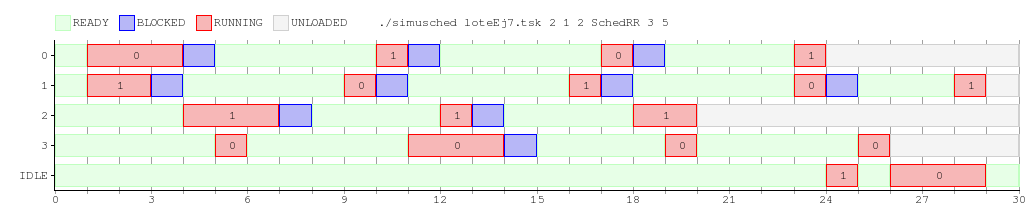
\includegraphics[scale=0.45]{../tp1/Test/resEj7Co2dis.png}
\\
\vspace{1pt}
\footnotesize\textit{Simulacro RR con dos n\'ucleos de quantum distintos}
\end{center}
\vspace{\baselineskip}

Como podemos observar los graficos son similares, esto radica en que si bien cuando aumentamos el quantum de uno de los nucleos tenemos la posibilidad de que un procesos se ejecute mas rapido, el mismo es afectado por los bloqueos realizados en la tarea corriendo.\\
Si nos basamos en la teoria, podemos decir que cuando el Scheduler corre con dos nucleos con la misma cantidad de quantum \textit{Fairness} es optimo ya que todos tendran las mismas posibilidades en tiempo de ejececucion, sin embargo, el mismo no es apropiado en el segundo caso, porque los procesos recibieran distintos quantums lo cual aletera esta metrica.\\
En el caso de \textit{Tiempo de Respuesta} va a mejorar en comparacion a el procesador con un nucleo ya que hay uno mas que puede ser utlizado, esto sucede en ambos casos.\\
Con respecto a \textit{Throughput} teniendo dos nucleos al menos 2 procesos pueden terminar por unidad de tiempo, lo cual mejora el primer experimento que solo perimitia uno.\\
En \textit{Turnaround} podemos decir que la mejora con respecto al primer experimento es que ademas de que algun proceso comenzara a ejecutarse antes ya que ahora  hay un nucleo mas, en el caso de quantums distintos, si el proceso arbitrariamente es beneficiado obteniendo el nucleo con mayor quantum terminara antes, mientras que los bloqueos no alteren su ejecucion.

\vspace{1 cm}
Por ultimo, observamos que pasaria si nuestro procesador tiene tres nucleos, al igual que el ultimo experimento realizado tenemos dos posibilidades, aqui las mismas:

\vspace{\baselineskip}
\begin{center}
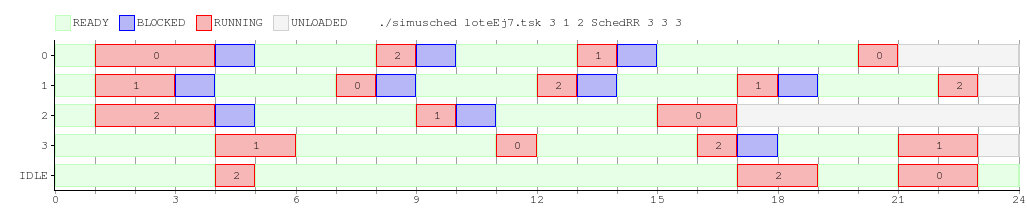
\includegraphics[scale=0.45]{../tp1/Test/resEj7Co3.png}
\\
\vspace{1pt}
\footnotesize\textit{Simulacro RR con tres n\'ucleos de quantum iguales a 3}
\end{center}
\vspace{\baselineskip}

\vspace{\baselineskip}
\begin{center}
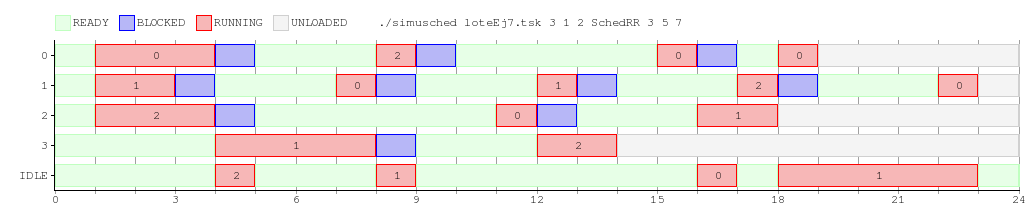
\includegraphics[scale=0.45]{../tp1/Test/resEj7Co3dis.png}
\\
\vspace{1pt}
\footnotesize\textit{Simulacro RR con tres n\'ucleos de quantum distintos}
\end{center}
\vspace{\baselineskip}

Para comenzar, las conclusiones que obtenemos, al igual que anteriormente son afectadas por los bloqueos que tiene los procesos.\\
Analicemos teoricamente nuestos experimentos.\\
En el caso de utlizar como metrica \textit{Fairness}, los resultados que obtenemos son iguales a los obtenidos en el segundo experimento. Es decir, en caso de poseer quantums iguales esta metrica es satifactoria, sin embargo, en el segundo caso no lo sera, ya que la CPU no esta brindandole una dosis justa a cada proceso.\\
Para \textit{Tiempo de Respuesta} obtenemos una mejora para este experimento con respecto al anterior, un proceso tiene posibilidades de comenzar a ejecutar mas tempranamente debido al aumento en la cantidad de nucleos. Aun siendo visible esta mejora claramente en quantums iguales, en el caso contrario tambien podemos notarlo, ya que al tener distintos quantums el procesador puede estar libre en distintos momentos.\\
Otra mejora que notamos es en el caso de utilizar como metrica \textit{Troughput} ya que con respecto a los experimentos anteriores, ahora podran finalizar al menos tres procesos en ambos casos.\\
Por último, si utilizamos \textit{Turnaround} podemos obetener una mejor medicion respecto a los ultimos dos experimentos. Esto es debido a que el procesaodr tiene tres nucleos, esto es mas notorio si ademas los quantums son distintos, ya que un proceso puede ser beneficiado obteniendo el nucleo con mayor tiempo y asi finalizar antes.

\vspace{0,5 cm}
Podemos concluir con estos experimentos que deducir que si un Scheduler es optimo varia segun algunos factores y que metrica estemos utilizando.\\
Pudimos ver que \textit{Fairness} depende de los quantums que se le asigna a cada nucleo del procesador, y segun eso puede resultar satifactorio o no.\\
En \textit{Tiempo de Respuesta} notamos que varia segun la cantidad de nucleos y, de tener distintos quantums, esto puede alterar los resultados aun mejor.\\
Para \textit{Troughput} depende de la cantidad de nucleos que tenga el procesador, ya que para que termine mas de una tarea, deben trabajar nucleos paralelamente.\\
Por ultimo, \textit{Turnaround} depende de varias cosas, en caso de que los quantums sean iguales no podemos concluir en demasiado, pero si tenemos disintos podemos obtener resultados satifactorios segun de cada proceso.\\
Si bien los resultados son teoricos, pudimos notar que nuestras medidas resultan alteradas por los bloqueos realzados por las tareas, el costo de la migracion de un nucleo a otro y el cambio de contexto.



>>>>>>> 63ea077d0c52c262c2910339492dcc2387679a4d
\subsection{Ejercicio 8: Round Robin sin migracion}

En este ejercicio implementamos un scheduler Round Robin  que no permite migraciones entre procesos, llamado RoundRobin2. Para lograr esto, mantenemos una
cola por procesador 
y un contador que controla cuantas tareas hay activas por cpu. Para asignar una tarea a un cpu, nos basta con recorrer los contadores 
y quedarnos con alguno
de los de valor minimo. Ademas, cada vez que una tarea se bloquea, almacenamos en una variable cual
es el procesador al que estaba asignada. De este modo, para todos los procesadores, podemos ejecutar como si fuera Round Robin comun. La diferencia
radica en que cuando una tarea se bloquea, se almacena el valor de cpu de la misma. Cuando la tarea se desbloquea, basta con buscar su
cpu y pushearla en la cola del mismo.

Vamos a comparar esta version del scheduler Round Robin con la presentada en el ejercicio 3. Los schedulers tiene diferente comportamiento solo en 
determinados casos, que son lo que vamos a analizar. Dejaremos los puntos en comun de lado, como por ejemplo, la rotacion total de las tareas.
Por lo tanto, compararemos la optimalidad en el uso de los procesadores. Es decir, compararemos la cantidad de tiempo de cpu despercidiado. 
Para esto correremos con dos procesadores el siguiente lote de tareas:
\begin{center}
TaskCPU 10\\
TaskCPU 5\\
TaskCPU 20
\end{center}
 La idea de es comparar cuanto tarda cada scheduler en completar el procesamiento total. Notese que pusimos la tarea de mejor ejucucion en el medio 
 aproposio. Asi forzamos al RR2 a usar un procesador unicamente para una tarea corta, mientras que debe usar el otro para dos tareas grandes.
 Es decir, estamos forzando un caso concreto para representar casos mas generales. Ademas, se debe tener el cuenta que el costo de migracion 
 es de 2 tick, lo cual es bajo teniendo en cuenta todos los datos que se podrian tener que duplicar.

\vspace{\baselineskip}
\begin{center}
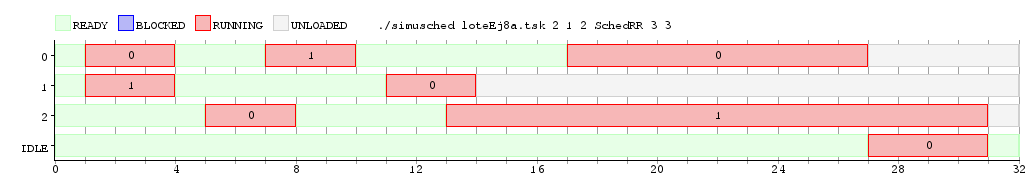
\includegraphics[scale=0.45]{../tp1/Test/resEj8Co2SBRR.png}
\\
\vspace{1pt}
\footnotesize\textit{Simulacro RR con 2 n\'ucleos de quantum 3.\\Con 2 tick de costo de migracion.}
\end{center}
\vspace{\baselineskip}

\vspace{\baselineskip}
\begin{center}
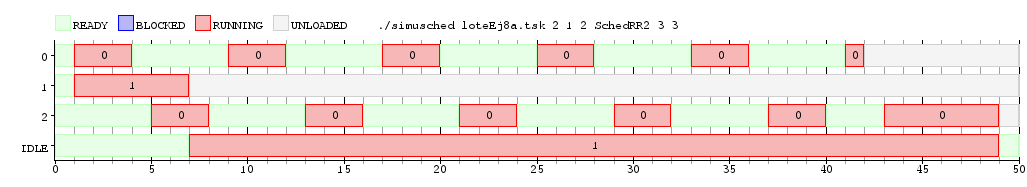
\includegraphics[scale=0.45]{../tp1/Test/resEj8Co2SBRR2.png}
\\
\vspace{1pt}
\footnotesize\textit{Simulacro RR2 con 2 n\'ucleos de quantum 3\\Con 2 tick de costo de migracion.}
\end{center}
\vspace{\baselineskip}

Como podemos observar, el tiempo para obtener la ejecucion total es mucho mayor en RR2, ya que no puede usar uno de los procesadores. 
\textquestiondown Pero que pasaria si el costo de migrar entre proesadores fuera mayor? Digamos, mas del doble del quantum...

\vspace{\baselineskip}
\begin{center}
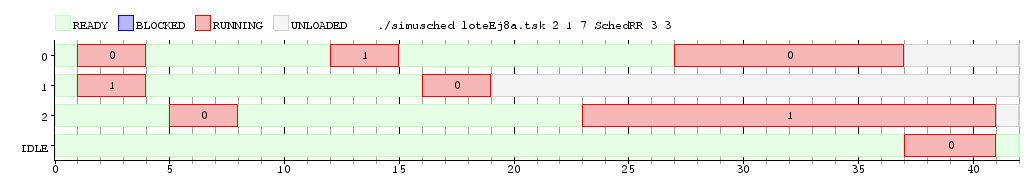
\includegraphics[scale=0.45]{../tp1/Test/resEj8Co2SBRRMM.png}
\\
\vspace{1pt}
\footnotesize\textit{Simulacro RR con 2 n\'ucleos de quantum 3.\\Con 7 tick de costo de migracion.}
\end{center}
\vspace{\baselineskip}

\vspace{\baselineskip}
\begin{center}
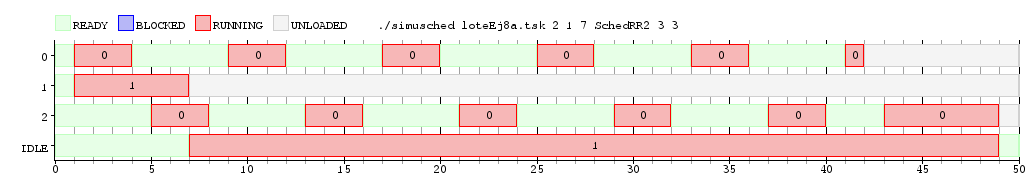
\includegraphics[scale=0.45]{../tp1/Test/resEj8Co2SBRR2MM.png}
\\
\vspace{1pt}
\footnotesize\textit{Simulacro RR2 con 2 n\'ucleos de quantum 3.\\Con 7 tick de costo de migracion.}
\end{center}
\vspace{\baselineskip}

Podemos notar que aunque la diferencia se redujo, el tiempo total de RR2 sigue siendo mayor que el de RR. Por lo tanto, solo nos resta concluir que 
no permitir migracion entre procesadores es un error. Esto sujeto a condiciones normales.  Si tuviesemos un costo de migracion ridiculamente alto, 
si trabajasemos fuera de la cache para la migracion, 
entonces deberia considerarse realizar una nueva experimentacion comparando los nuevos porcentajes.

\subsection{Ejercicio 9}

En este ejercicio, debimos idear un lote de tareas que cumpliera en simult\'aneo, las siguientes condiciones:

\begin{itemize}
 \item Tener un scheduling no factible para el algoritmo de prioridades fijas
 \item Tener un scheduling factible para el algoritmo de prioridades din\'amicas
\end{itemize}

El lote que propusimos para este experimento es el siguiente:

\begin{verbatim}
  lote.tsk:
    &A1,10,4
    &B3,4,1
\end{verbatim}

Es decir, una repetici\'on de tarea de tipo A, con 4 ciclos de clock de tiempo de ejecuci\'on y 10 ciclos de clock como per\'iodo, y 3 repeticiones 
de tareas de tipo B, con 1 ciclo de clock de tiempo de ejecuci\'on y per\'iodo igual a 4. A continuaci\'on, mostraremos que con esta combinaci\'on
de per\'iodos y tiempos de ejecuci\'on, la tarea A no terminar\'a de ejecutarse antes de su \textit{deadline} (ciclo de clock n\'umero 10) 
para el scheduler de prioridades fijas. Es importante notar que a los tiempos de ejecuci\'on de las dos familias de tareas hay que sumarle el ciclo
de clock extra correspondiente a la llamada a \textit{exit()}. Por lo tanto, la tarea A requerir\'a de 5 ciclos para completar su ejecuci\'on, y las tareas 
B requerir\'an de 2 ciclos cada una.

Veamos el diagrama de Gantt para este lote, con scheduling con prioridades fijas:

\vspace{\baselineskip}
\begin{center}
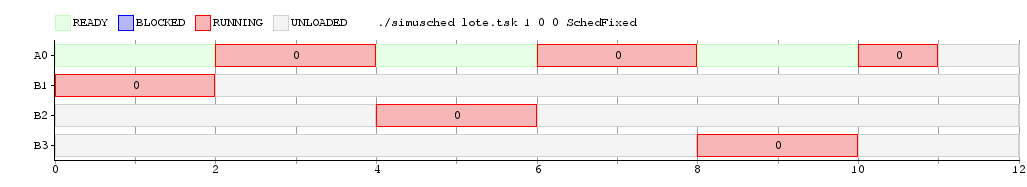
\includegraphics[scale=0.45]{../tp1/Test/ejercicio9-1.png}
\\
\vspace{1pt}
\footnotesize\textit{Simulaci\'on SchedFixed}
\end{center}
\vspace{\baselineskip}

En los instantes m\'ultiplos de 4 (0, 4 y 8) llega al sistema una \textit{request} por una tarea de familia B, mientras que en el instante 0 llega la \'unica 
\textit{request} por una tarea de tipo A. Como las tareas de tipo B, por tener menor per\'iodo, son m\'as prioritarias que la de tipo A, en los instantes
0, 4 y 8, el scheduler decide poner a correr las tareas de tipo B, durante los dos ciclos que necesitan para terminar. Esto le deja a la tarea A
4 ciclos de clock disponibles en los primeros 10 ciclos de clock, con lo cual no puede terminar la ejecuci\'on antes de que llegue su deadline,
haciendo inviable el uso del scheduler de prioridades fijas para este lote de tareas.
\\
Ejecutando el mismo lote de tareas, pero con scheduling de prioridades din\'amicas, obtenemos el siguiente diagrama de Gantt:

\vspace{\baselineskip}
\begin{center}
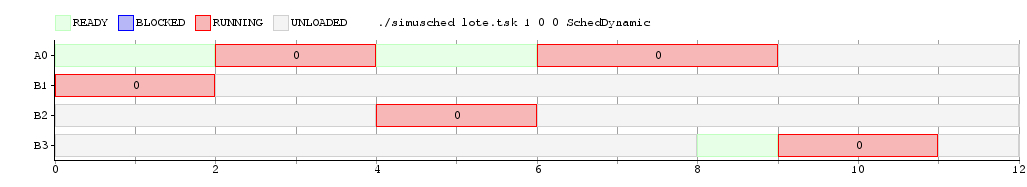
\includegraphics[scale=0.45]{../tp1/Test/ejercicio9-2.png}
\\
\vspace{1pt}
\footnotesize\textit{Simulaci\'on SchedDynamic}
\end{center}
\vspace{\baselineskip}

En esta simulaci\'on, el comportamiento del scheduler es id\'entico al de prioridades fijas hasta el instante 8, correspondiente a la tercer \textit{request}
por una tarea de tipo B. En este instante, la tarea de tipo A tiene su deadline dentro de 2 ciclos de clock, mientras que la tarea de tipo B tiene
su deadline a 4 ciclos de clock de distancia, por lo cual el scheduler decidir\'a poner a correr a la tarea de tipo A en vez de la tarea de tipo B.
Esto le permitir\'a a la tarea de tipo A consumir el \'ultimo ciclo de CPU que necesitaba, y luego el scheduler pondr\'a a correr a la \'ultima
tarea de tipo B, que terminar\'a sin problemas su ejecuci\'on. As\'i, todas las tareas del lote terminaron su ejecuci\'on antes de su \textit{deadline}.
